\section{Evaluation}
\label{SEC:evaluation}

To be able to evaluate how CrashSimulator performs, a series of tests were
conducted using a prototype build on {\tt rr} version 5.2.0 running on a
32-bit Linux kernel running distributed with  Ubuntu 16.04 LTS.  Our
modifications to {\tt rr} were carried out in C++ and the CrashSimulator
supervisor was implemented in ZZZZ lines of Python 2.7 code with a YYYY
line C extension that allows it to interact with processes using the {\tt
Ptrace} API.  This version of CrashSimulator is available as a Docker
container and, due to some operating system configuration being necessary,
is most easily installed in this fashion.

For a test environment, we chose
a vmware virtual machine running version of CrashSimulator described above.
We ran the tests on a 1.7 gHz
core i7 system with 8GB of RAM. Our implementation used {\tt ptrace} to
interpose on the running program and interject anomalous behavior into its
execution.  To our knowledge, the only major negative impact of
these design choices was that the use of {\tt ptrace} and Python did slow
down our
prototype's performance.  On the positive side, it simplified construction.
As will be discussed later, much of this performance
degradation is offset by the highly asynchronous fashion in which our
prototype can execute tests.

Part of our evaluation consisted of a user study involving
YYYY participants from a computer science master's
program.  These students had varying backgrounds in relation to software
development and automated testing.  All received AAA hours
of training on CrashSimulator.  This training focused on the tools'
initial setup, configuration, and usage,
as well as on how to interpret its
results.

We asked our participants to test popular real-world applications with the
goal of identifying new bugs and reporting them to the application's
developers.  In performing this task our participants had to correctly set
up and configure CrashSimulator, execute a testing process, evaluate the
results, and produce a sufficient proof of validity for each bug to
convincingly support the case for fixing it.
To focus this process on the actual but finding and fixing
process, rather than open source development meta-concerns, participants
were encouraged, but not limited to, testing applications listed highly on
the Debian popularity contest.  These applications are more likely to have
clean, mature code bases and active developer communities reducing the
barrier to entry for our participants.

We used three techniques to capture the experience of our participants as
they used the tool.  First, we examined the time required for participants
to perform each step of the process of finding and reporting a bug.
This data, along with hard counts of the number of bugs identified by our
participants using each of the tools, provided a quantitative measure of
each tool's usability.

To measure qualitative concerns,
participant impressions were gathered using
several instruments.  First, data on developer skills and educational
backgrounds was gathered using a pre-study survey.
Second, during the three week
study period, the participants' progress toward finding and fixing bugs was
tracked through the submission of weekly update worksheets.  Finally, at
the end of the study period, overall developer impressions were gathered
using a post-survey and one-on-one interviews.  These instruments were
structured to give insight into CrashSimuator's usability, extendability, and
overall effectiveness at finding bugs.

With our prototype and study instruments in hand, we
set out to answer the following questions:

\begin{enumerate}

\item{Can CrashSimulator find environmental bugs in widely used applications?
(Subsection~\ref{sec-env-bugs})}

\item Does CrashSimulator allow its users to efficiently construct a test suite?

\item Does CrashSimulator provide output that is useful in locating and
fixing bugs?

\item{Do tests using CrashSimulator make yield too many false positives?
      (Subsection~\ref{sec-sorts-errors})}

\item{Can CrashSimulator
      execute tests efficiently? (Subsection~\ref{sec-perf})}

\end{enumerate}

\subsection{Can CrashSimulator find environmental bugs in widely used
applications?}
\label{sec-env-bugs}

The most crucial question to ask about CrashSimulator is whether or not it is
effective in finding new environmental bugs in popular applications.
identified by CrashSimulator exist in in popular applications?  If it cannot
find such bug then there is little reason for CrashSimulator to exist.
To test this premise,
we chose to look for two anomalies that we could test for in a large
array of programs.  One is a file system anomaly and the other is found in
network applications.
However, both use common API calls, and thus had the potential to
appear in many programs.  We selected the tested applications either
because they were deemed
``popular'' by Debian's Popularity Contest~\cite{DebPopCon}, or were from
GNU Coreutils.  Coreutils applications were chosen because of their
widespread inclusion in many Linux distributions.

\subsubsection{Unexpected File Types}
\label{sec-file-type-bugs}
Providing unexpected types of files to
applications.

The first anomaly investigated occurs when an application has to retrieve
and process data from a file.  Linux supports several ``special'' file
types apart from the standard ``regular'' file type, such as
directories, symbolic links, character devices, block devices, sockets, and
First-In-First-Out (FIFO) pipes.  While these special files
use the same system calls as regular files (such as {\tt read()} and
{\tt write()}), they behave in very different ways.  For example, {\tt
/dev/urandom} is a character device that produces an infinite amount of
pseudo-random data when read.  If an application that reads the full
contents of a file before processing it is provided {\tt /dev/urandom}, it
will fill memory or disk space and could
crash the system~\cite{YumAptEndless}.
Correct execution in these situations often requires applications
to examine the files in order to ensure they are of an appropriate type.

{\bf Method.}  Identifying these bugs involves changing an application's
execution trace to induce its response to an unexpected file type.  For
example, the {\tt sed} application, which modifies the contents of a text
file according to a provided command string, could be provided a symbolic
link, a directory, or a character device instead.  CrashSimulator
accomplishes this by identifying the calls to {\tt stat()}, {\tt fstat()},
or {\tt lstat()} that an application makes to examine the file, and then
changes the trace to simulate
one of the special file types.  If the application responds to
this injected information then there is the possibility that the special
file will be handled correctly.  On the other hand, if there is no
alteration in the behavior of the application,  then the condition is not
being handled correctly.

{\bf Findings.}
The results of this round of tests were shown in
Table~\ref{table:unexpectedtypes}.

For each application, CrashSimulator was invoked multiple times,and
the trace was modified
to simulate each of the non-standard file type anomalies.  Some
of the applications opened multiple files; in these cases each anomaly was
simulated for each of the file arguments to the application.
Table~\ref{table:unexpectedtypes} also shows the values that CrashSimulator
inserts into the return value of the {\tt stat()}-like call,
in response to
different file type anomalies.  A result of ``Initial Value'' indicates
that this is the file type the application was provided when the replayed
execution trace was recorded -- that is, a file of the type the application
was expecting.  A result of ``Recognizes'' indicates that the application
identified that it was being provided with an unexpected file type and its
execution diverged, indicating that it was potentially handling the
unexpected file type correctly.  A result of ``Fail'' indicates that the
application failed to recognize the presence of the unusual file type
because execution never diverged from the trace being replayed.  We
manually examined a subset of the listed application behaviors simulated by
CrashSimulator and verified they were consistent with the actual behavior
on the given file type.

\begin{table*}[t]
    \scriptsize{}
    \begin{tabular}{l  l  |  l  l  l  l  l  l  l}
    \toprule{}
        Application & Condition Tested           & IFREG        & IFDIR        & IFCHR     & IFBLK    & FIFO      & IFLNK    & IFSOCK\\
\hline
        {\tt Aspell}      & Dictionary File            & Initial Value  & Fail           & Recognizes  & Fail       & Fail        & Fail       & Fail\\
        {\tt Aspell}      & File being checked         & Initial Value  & Fail           & Recognizes  & Fail       & Fail        & Fail       & Fail\\
        {\tt gnu-gpg}     & secring.gpg                & Initial Value  & Fail           & Fail        & Fail       & Fail        & Fail       & Fail\\
        {\tt vim}         & File being opened          & Initial Value  & Recognizes     & Recognizes  & Recognizes & Recognizes* & Recognizes & Fail\\
        {\tt nano}        & File being opened          & Initial Value  & Recognizes     & Recognizes  & Recognizes & Fail        & Fail       & Fail\\
        {\tt sed}         & File being edited          & Initial Value  & Fail           & Recognizes  & Fail       & Fail        & Fail       & Fail\\
        {\tt df}          & /proc                      & Fail           & Initial Value  & Fail        & Fail       & Fail        & Fail       & Fail\\
        {\tt wc}          & File being checked         & Initial Value  & Recognizes     & Recognizes  & Recognizes & Recognizes  & Recognizes & Recognizes\\
        {\tt du}          & Directory being checked    & Recognizes     & Initial Value  & Recognizes  & Recognizes & Recognizes  & Recognizes & Recognizes\\
        {\tt install}     & File being installed       & Initial Value  & Recognizes     & Fail       & Fail      & Fail       & Recognizes & Fail\\
        {\tt fmt}         & File being formatted       & Initial Value  & Fail          & Recognizes  & Fail      & Fail       & Fail      & Fail\\
        {\tt od}          & File being dumped          & Initial Value  & Fail          & Recognizes  & Fail      & Fail       & Fail      & Fail\\
        {\tt ptx}         & File being read            & Initial Value  & Recognizes     & Recognizes  & Recognizes & Recognizes  & Recognizes & Recognizes\\
        {\tt comm}        & Second file being compared & Initial Value  & Fail           & Recognizes  & Fail       & Fail        & Fail       & Fail\\
        {\tt pr}          & File being read            & Initial Value  & Fail           & Fail        & Fail       & Fail        & Fail       & Fail\\
\hline
        {\tt readlink}    & Link being evaluated       & \textbf{No file checks performed} & & & & & & \\
        {\tt unlink}      & File being unlinked        & \textbf{No file checks performed} & & & & & & \\
    \bottomrule{}
    \end{tabular}
    \caption{Applications tested for their handling of unexpected file types.}
    \label{table:unexpectedtypes}
\end{table*}

The frequency of failed executions in our results indicate that many
applications make the assumption that they will only be used to process
regular files.  When this assumption does not hold, execution results
can be hard to predict.  In many cases a denial of
service condition occurs in the form of the application ``hanging,'' as it
attempts to incorrectly process the file.  This may happen harmlessly, such
as if an application blocks forever waiting for a {\tt read()}
call to retrieve non-existent data from an empty FIFO, or harmfully, as
when an application attempts to read in and process an
``infinitely large'' file, that will eventually fill all
available memory or disk
space~\cite{Cappos_CCS_08}.

Of particular interest is the behavior we see in the last two applications
listed in Table~\ref{table:unexpectedtypes}.  Each application correctly
recognized when an unexpected file type was encountered, as they
are simply ``dumb'' wrappers around the system calls
with which they share a name.  As such, they essentially,
they just hand the specified
file to their corresponding system call and, in the case of an error, use
{\tt perror()} to print the correct localized error message.  In short,
these applications pass their error handling responsibilities to the
kernel.

\begin{table}[t]
    \scriptsize{}
    \begin{tabular}{l  l  l  l  l  l  l  l  l}
    \toprule{}
        Application         & IFDIR                     & IFCHR       & IFBLK                & FIFO \\
\hline
        {\tt wc}            & Error: Is a Directory     & hangs       & slowly process file  & Hangs\\
        {\tt install}       & Error: Omitting Directory & Fills disk  & slowly copies file   & Hangs\\
        {\tt fmt}           & No output                 & hangs       & garbage output       & Hangs\\
        {\tt od}            & Error: read error         & hangs       & No output            & Hangs\\
        {\tt ptx}           & Error: Is a Directory     & fills disk  & garbage output       & Hangs\\
        {\tt comm}          & Error: Is a Directory     & hangs       & garbage output       & Hangs\\
        {\tt pr}            & Error: Is a Directory     & hangs       & garbage output       & Hangs\\
\hline
    \bottomrule{}
    \end{tabular}
    \caption{Responses of a sample of coreutils applications when exposed to
      anomalous conditions.  The IFCHR file used was the infinite-length {\tt
        /dev/urandom}.}
    \label{table:applicationresponses}
\end{table}


In order to confirm the accuracy of CrashSimulator's assessments we manually
exposed a subset of the Coreutils applications we tested to the unusual file
types to get an idea of how they would respond.
Table~\ref{table:applicationresponses} contains the results of this test.
CrashSimulator's evaluation of an application can map to real world bug behavior
in a few different combinations
One
possibility is that CrashSimulator asserts that the application will fail
and in practice it does.  This is the case when we evaluated
the response of  {\tt install} when it was provided a character device
rather than a regular file. CrashSimulator predicted failure and the
application ended up filling the disk of the machine on which it was run.  The
opposite can also occur.  That is, CrashSimulator reports that the
application detected the anomalous condition and the application manages to
do so in practice,  as when we evaluated {\tt wc}'s response to
being run on a directory.

There were however, a few times when CrashSimulator and the
application's response disagreed.  This
happened when we evaluated {\tt ptx}'s response to an
infinite-sized character device.  CrashSimulator reported that {\tt ptx}
had correctly responded to the anomaly.  But in reality, {\tt ptx} filled the
disk of the the test machine.  As will be discussed later, correcting this
error is easily accomplished by improving the checker used in this
assessment -- an effort similar to updating a unit test when it is shown to
be incomplete.  Overall, the results of this ``real world'' analysis
support the claim that CrashSimulator can identify real bugs that can have
damaging consequences.

\subsubsection{Slowloris attack} Delaying network applications for extended
periods.


The second anomaly we examined involves an application's behavior when it
attempts to communicate over a network with extremely long (on the order of
minutes) response times.  At a low level, applications retrieve data from a
network socket by waiting for data to be available and then reading it.  A
key aspect of this approach is handling the situation where communication
takes too long and should time out.

{\bf Method.} CrashSimulator can detect whether an application is
vulnerable to this attack by modifying the trace to simulate large
amounts of time elapsing between network operations.  In this approach,
CrashSimulator determines whether or not the application makes any effort
to configure its network communications with a timeout value. This is done
by examining the presence or absence of {\tt setsockopt()}, {\tt poll()}
and {\tt select()} calls as well as the timeout values that may or may not
have been passed to them. Applications that do not set the timeout are
subject to the operating system-defined protocol timeout value (19 minutes
on Linux).  Note that by properly manipulating the results of all
time-returning calls, CrashSimulator can simulate an execution where close
to the maximum timeout value occurs, without actually spending any time
waiting.


Again, our selection of network applications and libraries were based on
those that were
most popular on Debian's ratings~\cite{DebPopCon}.

\begin{table}[t]
  \scriptsize{}
  \begin{tabular}{l | l}
    \toprule{}
    {\bf Application}              & {\bf Analysis Result}\\
    {\tt wget}                     & Overly long timeout supplied to {\tt select()} \\
    {\tt ftp}                      & No {\tt poll()} or {\tt select()}, no timeout set \\
    {\tt telnet}                   & {\tt select()} specifies no timeout \\
    {\tt urllib http}              & No {\tt poll()} or {\tt select()}, no timeout set \\
    {\tt urllib ftp}               & No {\tt poll()} or {\tt select()}, no timeout set \\
    {\tt ftplib}                   & No {\tt poll()} or {\tt select()}, no timeout set \\
    {\tt httplib}                  & No {\tt poll()} or {\tt select()}, no timeout set \\
    {\tt requests}                 & No {\tt poll()} or {\tt select()}, no timeout set \\
    {\tt urllib3}                  & No {\tt poll()} or {\tt select()}, no timeout set \\
    {\tt python-websocket-client}  & No {\tt poll()} or {\tt select()}, no timeout set \\
    \bottomrule{}
  \end{tabular}
  \caption{Applications tested for their handling of extremely slow response
    times from the host with which they are communicating }
  \label{table:slowloris}
\end{table}


{\bf Findings.} As Table~\ref{table:slowloris} shows, all of these
applications were vulnerable to this sort of anomaly, with timeouts taking
hours or even days in some cases to resolve.
What's more, in the vast majority of
cases, the problem occurs because the application makes no effort to
specify a timeout value.  This means an attacker can transmit one byte of
data per timeout period (per Linux's value of 19 minutes for TCP sockets),
allowing them to keep the application alive instead of quitting.


This attack technique has been effectively exploited in the wild.  The {\tt
slowloris} tool allows a single attacking host to successfully deny service
to a vulnerable web server with minimal bandwidth usage by simply
introducing delays between the headers sent to the victim by an attacking
HTTP client.  Because many web servers at the time  of {\tt slowloris's} release
allowed large timeouts
between messages from the clients, one web client could effectively tie up
the resources of a web server for a long period of time.
This can cause a slow buildup of unending or long lived jobs that consume
resources and cause detrimental system behavior~\cite{Slowloris}.
Similar attacks can be used to indefinitely delay security updates to
clients, leaving them vulnerable to compromise~\cite{Cappos_TR_08}.


\subsubsection{Bugs Found By Participants}

Another topic of relevance in answering this question is how well new users are
able to find bugs with CrashSimulator.
To answer this question we can examine the bug finding results from our user
study.
A total of 15 bugs were found using CrashSimulator, and, perhaps not
surprisingly, the majority were reported by participants with a
self-reported high degree of operating systems experience.
~\ref{table:fig-tool-exp} contains the
counts of bugs identified during the study broken down by
the tool used to identify them, as well as developer's self reported
developer experience level with operating system concepts.
Participants with a moderate and low degrees of operating
systems experience found more bugs had success even if they found a lower total
volume of bugs.

{\bf Discussion. }

The above results indicate that, when it comes to using CrashSimulator,
having experience with operating systems concepts is very beneficial.  At
the same time, users with a self-reported low degree of experience with OS
concepts were still able to identify bugs by using its built in corpus of
anomalies. ~\ref{table:fig-tool-anomaly} shows which
of these anomalies most commonly
resulted in application bugs.

\begin{figure}[t]
  \center{}
  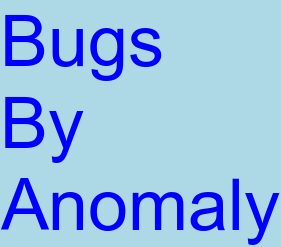
\includegraphics[scale=.5]{images/anomaly}
  \caption{\emph{Bugs Found Using CrashSimulator Organized by Anomaly}}
  \label{fig-tool-anomaly}
\end{figure}

{\bf Concluding Thoughts} The results of the above analysis show that
CrashSimulator is readily able to identify novel bugs in widely used
applications, including security-focused applications like gnu-gpg, and a host
of popular network applications, by following a repeatable and principled
protocol.


\subsection{Does CrashSimulator allow its users to construct a test suite
efficiently?}

While CrashSimulator is able to test an application's response to a suite
of anomalies out of the box its capabilities can be extended to best fit
the needs of its users.  To get an idea of what end users might do with
this functionality we asked our study participants to identify a new
anomaly, construct a mutator for it, and test real world applications
against it.
The effort and skill involved in
this process is similar to that involved in writing a unit test or
integration test using a modern testing framework.  However, unlike a unit
test or integration test, a CrashSimuator test can be run
against multiple
applications without concern for dependencies like the language in which
they were
written in or the libraries they depend on allowing its users to get more
value for the effort they put in.


{\bf Findings. }

Participants were split in the value they received
from their attempts to extend
CrashSimulator.  Of the ZZZ participants, YYY were able to complete the
process of identifying and adding an environmental anomaly to
CrashSimulator.  Of these BBB went on to identify new bugs using the novel
anomalies.  However, NNN were unable to complete this process.  Survey
results indicate that the process of identifying an anomaly stymied the
majoity of this group.

There was a consensus that
CrashSimulator required a
moderately high initial outlay of effort before testing could begin.
Surveys indicated that participants indicated that
adding a new anomaly to
CrashSimulator was more difficult than adding a new unit test to an
existing test suite.
However, the participants
appreciated
CrashSimulator's ability to allow for
testing
across multiple applications
with minimal additional effort once the tests had been constructed.

There was a great deal of
positive feedback around CrashSimulator's ability to use a mutator to apply
an anomaly to multiple eligible system call sequences throughout an
execution.  This meant a single test could be constructed to cover similar
operations throughout an application's code base, which would
shrink the size of the
required test suite in the process.


{\bf Discussion. }

Examining survey results
shows that previous operating system experience predicts more success in
adding anomalies to CrashSimulator.  This is unsurprising as a developer
inexperienced in these concepts would likely struggle to both identify
a new anomaly and its effects in terms of system call results and side
effects.
Previous experience with automated testing was also indicative of success.
Several participants that did not have experience in this area struggled
reported being bogged down in the process of putting together new mutators
and evaluating their correctness.  These results are encouraging in light
of the limited length of the study.  We believe that as developers become
more proficient with the CrashSimulator the difficulties some of our
participants experienced will be alleviated.


\subsection{Does CrashSimulator provide output that is useful in locating
and fixing bugs?}


{\bf Findings. }

Identifying the code responsible for a bug can present a major challenge in
large, complex applications.  By nature of its operation CrashSimulator is
able to provide a specific sequence of system calls responsible for a
failed test.  This can provide developers with a solid starting point as
they work to diagnose the cause of application misbehavior.
Participant feedback across the board indicated that CrashSimulator's
output made it assisted in identifying the source of bugs identified with
the tool.  This assertion is backed up by the high percentage of identified
bugs that ended up being successfully diagnosed and fixed by our survey
participants.  Specific counts are available in the table
~\ref{table:fig-fixed-tool} that
shows a high percentage of bugs identified with
CrashSimulator were fixed.


\begin{figure}[t]
  \center{}
  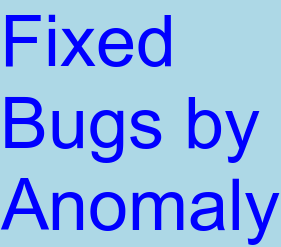
\includegraphics[scale=.5]{images/table3}
  \caption{\emph{Identified Bugs With Accepted Fixes.  This table needs
  to be updated}}
  \label{fig-fixed-tool}
\end{figure}


{\bf Discussion. }

There are two reasons, other than output quality, that bugs found with
CrashSimulator were likely to be fixed -- bug "depth" and the ease
with which a bug can be fixed.
It is possible that, because CrashSimulator
focuses on anomalies in an applications environment, a source of bugs that
is not well tested in most applications, a higher number of easily fixed,
low
hanging fruit style bugs were identified.
Additionally, many of the bugs types identifiable with CrashSimulator arise
because of a minor missing check meaning that the fix is small and easily
incorporated.

\subsection{What sorts of errors does CrashSimulator make?}
\label{sec-sorts-errors}

The primary source of false positives in CrashSimulator is an application
using a different sequence of system calls to implement a given operation
than a mutator was anticipating. CrashSimulator's approach allows these
situations to be easily corrected, once identified through analysis of the
incorrect test results.  This is similar to the circumstance where an
application's test suite is missing a test, necessitating action by the
developer to construct the missing test.

For example, consider GNOME's {\tt glib} file handling facilities.  When an
application makes use of these facilities to move a file across storage
devices the library itself correctly performs a
file move operation.  When we used CrashSimulator with
mutators that expected a calls to {\tt read()} and {\tt write()}
for a cross-device move, we got reports stating that the
application {\em did not} perform the system calls necessary to inject
an anomaly.  By manually
examining a system call trace, we found that, while {\tt glib} correctly
performs the requested move operation,
it does so using alternative system call
sequences.  Rather than using a sequence of {\tt read()} and {\tt write()}
calls, as our mutator expected, {\tt glib} creates a pipe and uses the {\tt
splice()} system call to copy the contents out of the source file, through
the pipe and into the destination file.

Fortunately, as soon as issues like this are discovered,
CrashSimulator's mutators can be modified to deal with alternative
approaches to handling an anomaly.  This approach is viable because there
are a finite number of system calls, and a given operation can be mapped to
a manageable subset of system calls.  Given the above example around moving
files, consider the mapping from high level ``operation'' to the set of
system calls that can implement it in Table~\ref{table:stepsandcalls}.
Each of the steps in the operation map to a small number of system calls
and, in most cases, only one of these system calls is necessary.  In
situations where two system call sequences can correctly implement the same
operation, CrashSimulator simply runs two checkers in parallel and accepts
the execution if either one ends in an accepting condition.

\begin{table}[t]
    \scriptsize{}
    \begin{tabular}{l | l }
    \toprule{}
      {\bf Operation}                                               & {\bf Potential System calls}\\
      Examine source file                                     & stat64(), lstat64(), fstat64()\\
      Examine destination file                                & stat64(), lstat64(), fstat64()\\
      Open source file                                        & open()\\
      Read contents of source file                            & read(), splice() with a pipe\\
      List source file's & \\ ~~~~~extended file attributes             & listxattr(), llistxattr(), flistxattr()\\
      %Read contents of source file's extended file attributes & getxattr(), lgetxattr(), fgetxattr()\\
      Read contents of source file's                    & \\
      ~~~~~~~extended file attributes & getxattr(), lgetxattr(), fgetxattr() \\
      Open destination file                                   & open(), optionally unlink() the file first\\
      Write contents to destination file                      & write(), splice() with a pipe\\
      Apply extended file attributes to & \\ ~~~~~destination file      & setxattr(), lsetxattr(), fsetxattr()\\
      Apply proper timestamps to & \\ ~~~~~destination file             & utimens(), futimens()\\
      Apply proper permissions & \\ ~~~~~to destination file            & chmod(), open() with a modeline specified\\
      Close the source file                                   & close()\\
      Close the destination file                              & close()\\
    \bottomrule{}
    \end{tabular}
    \caption{Each step of a successful cross-disk file move operation mapped to
      the system call or calls that can implement it}
    \label{table:stepsandcalls}
\end{table}

\subsection{Can CrashSimulator execute tests efficiently?}
\label{sec-perf}

One key attribute of successful testing tools is that they are able to
complete their tests in a timely manner.  If a tool takes too long
, users will be less likely to run it, which reduces its
usefulness dramatically. To this end, the performance of CrashSimulator was
evaluated in order to determine whether or not it was able to complete its
test executions in an acceptable time frame.

{\bf Method.} To determine the efficiency of CrashSimulator as a testing tool,
we examined the completion
times for executions of the specified application in both
native and replay execution modes.


    \begin{figure}[t]
        \center{}
        \fbox{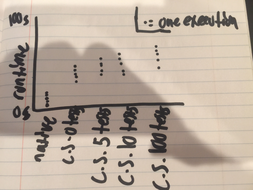
\includegraphics[scale=.75]{performance.png}}
        \caption{\emph{This shows the run time difference between the
native program and CrashSimulator in seconds.  Each dot indicates an
        execution.  The X axis shows time values for native executions, and
        executions under CrashSimulator with 0, 5, 10, and 100 tests
        performed respectively.
}}
         \label{figure:performance}

    \end{figure}


{\bf Findings.} Overall, the performance of CrashSimulator is usually
about an order of magnitude slower than if the original program is executed
natively.  This is largely due to performance problems in our (unoptimized)
prototype, primarily our utilization of Python and {\tt ptrace} once
process sets have been liberated from {\tt rr}.  Tracing the program
with {\tt ptrace} adds up to a factor of 5x in overhead,  which could be
removed with more efficient mechanisms like {\tt eBPF} or a loadable kernel
module.  In addition, starting up the Python interpreter increases the
startup time of our prototype's supervisor.

Though aspects of our performance were less efficient than desired, its
ability to execute many tests throughout the course of one replay and the
lack of blocking while waiting for test completion somewhat makes up for
this slowness. In some cases CrashSimulator will be more efficient than
running the program natively since {\tt rr's} replay does not require
actual execution of most system calls.  This means that CrashSimulator
avoids the system call overheads, such as I/O.

\preston{We probably want to keep this point, but I agree that it doesn't fit
here}
Note also that natively testing the timeout of networked applications (not
shown) would take an extended period of time, at least as long as the
allowed timeout value.  CrashSimulator avoids this cost by simulating the
fact that time has progressed for future system calls.

Overall, these results indicate that CrashSimulator is able to replay
executions in a performant manner.  Figure~\ref{figure:performance} shows
that the majority of the above executions completed around an order of
magnitude slower than their native counterparts.  CrashSimulator's
asynchronous testing means that enabling additional tests does not
significantly degrade performance as long as multiprocessing resources are
available on the system.
